%%%%%%%%%%%%%%%%%%%%%%%%%%%%%%%%%%%%%%%%%%%%%%%%%%%%%%%%%%%%%%%%%%%%%%%%%%%%%%%%
%2345678901234567890123456789012345678901234567890123456789012345678901234567890
%        1         2         3         4         5         6         7         8

\documentclass[letterpaper, 10 pt, conference]{ieeeconf}  % Comment this line out if you need a4paper
%\documentclass[a4paper, 10pt, conference]{ieeeconf}      % Use this line for a4 paper

\IEEEoverridecommandlockouts                              % This command is only needed if 
                                                          % you want to use the \thanks command

\overrideIEEEmargins                                      % Needed to meet printer requirements.

% See the \addtolength command later in the file to balance the column lengths
% on the last page of the document

% The following packages can be found on http:\\www.ctan.org
\usepackage{graphics} % for pdf, bitmapped graphics files
\usepackage{epsfig} % for postscript graphics files
\usepackage{mathptmx} % assumes new font selection scheme installed
\usepackage{times} % assumes new font selection scheme installed
\usepackage{amsmath} % assumes amsmath package installed
\usepackage{amssymb}  % assumes amsmath package installed
% \usepackage{comment}
% \usepackage{algorithm,algpseudocode}
% \usepackage{resizegather}
% \usepackage{flexisym}
\usepackage{dblfloatfix}    % To enable figures at the bottom of pag
\usepackage{subcaption}
\usepackage{mathtools}

% TODO: french letter in name
% \usepackage{inputenc} 

\title{\Large \bf Social RL: Socially Compliant Navigation in Crowds
with Reinforcement Learning}

\author{% <-this % stops a space
\thanks{This work was supported by [?]}% <-this % stops a space
% \thanks{$^{1}$L is with, 
% {\tt\small b.d.researcher@ieee.org}}%
% \thanks{$^{*}$Equal contribution}       
\thanks{Visual Intelligence for Transportation Laboratory, Ecole Polytechnique Federale de Lausanne (EPFL)
, CH-1015 Lausanne,
        {\tt\small \{ \}@epfl.ch}}%
}

\begin{document}

\bstctlcite{IEEEexample:BSTcontrol}

\maketitle
\thispagestyle{empty}
\pagestyle{empty}

\pdfminorversion=4  
%%%%%%%%%%%%%%%%%%%%%%%%%%%%%%%%%%%%%%%%%%%%%%%%%%%%%%%%%%%%%%%%%%%%%%%%%%%%%%%%
\begin{abstract}
This electronic document is a template. The various components of your paper [title, text, heads, etc.] are already defined on the style sheet, as illustrated by the portions given in this document.

\vspace{5cm}

\end{abstract}


%%%%%%%%%%%%%%%%%%%%%%%%%%%%%%%%%%%%%%%%%%%%%%%%%%%%%%%%%%%%%%%%%%%%%%%%%%%%%%%%
\section{INTRODUCTION} \label{sec:intro}

With the rapid growth of machine intelligence, robots are envisioned to expand habitats from isolated environments to social spaces that are shared with humans and other embodied agents. Traditional approaches for robot navigation often view the moving agents nearby as a static obstacle \cite{fox_dynamic_1997} or react to them through a one-step lookahead \cite{berg_reciprocal_2008}, resulting in short-sighted and unnatural behaviors. In order to navigate through a crowd in a socially compliant manner, robots need the ability to understand the behaviors of the others while making its movement decision. 

Navigation with social etiquettes is, however, a very challenging task. As communications among agents (e.g. robots, pedestrians, bikers) are not widely available, robots need to perceive and anticipate the evolution of the crowd that can involve complex interactions. Research works in trajectory prediction have proposed several hand-crafted or data-driven methods to model the agent-agent interactions \cite{helbing_social_1995,alahi_social_2016,vemula_social_2017,gupta_social_2018}. In a addition to the predictive model, how to integrate the interaction knowledge into the decision-making process poses another challenge as well. 

\begin{figure} [h]
  \captionsetup{font=small}
  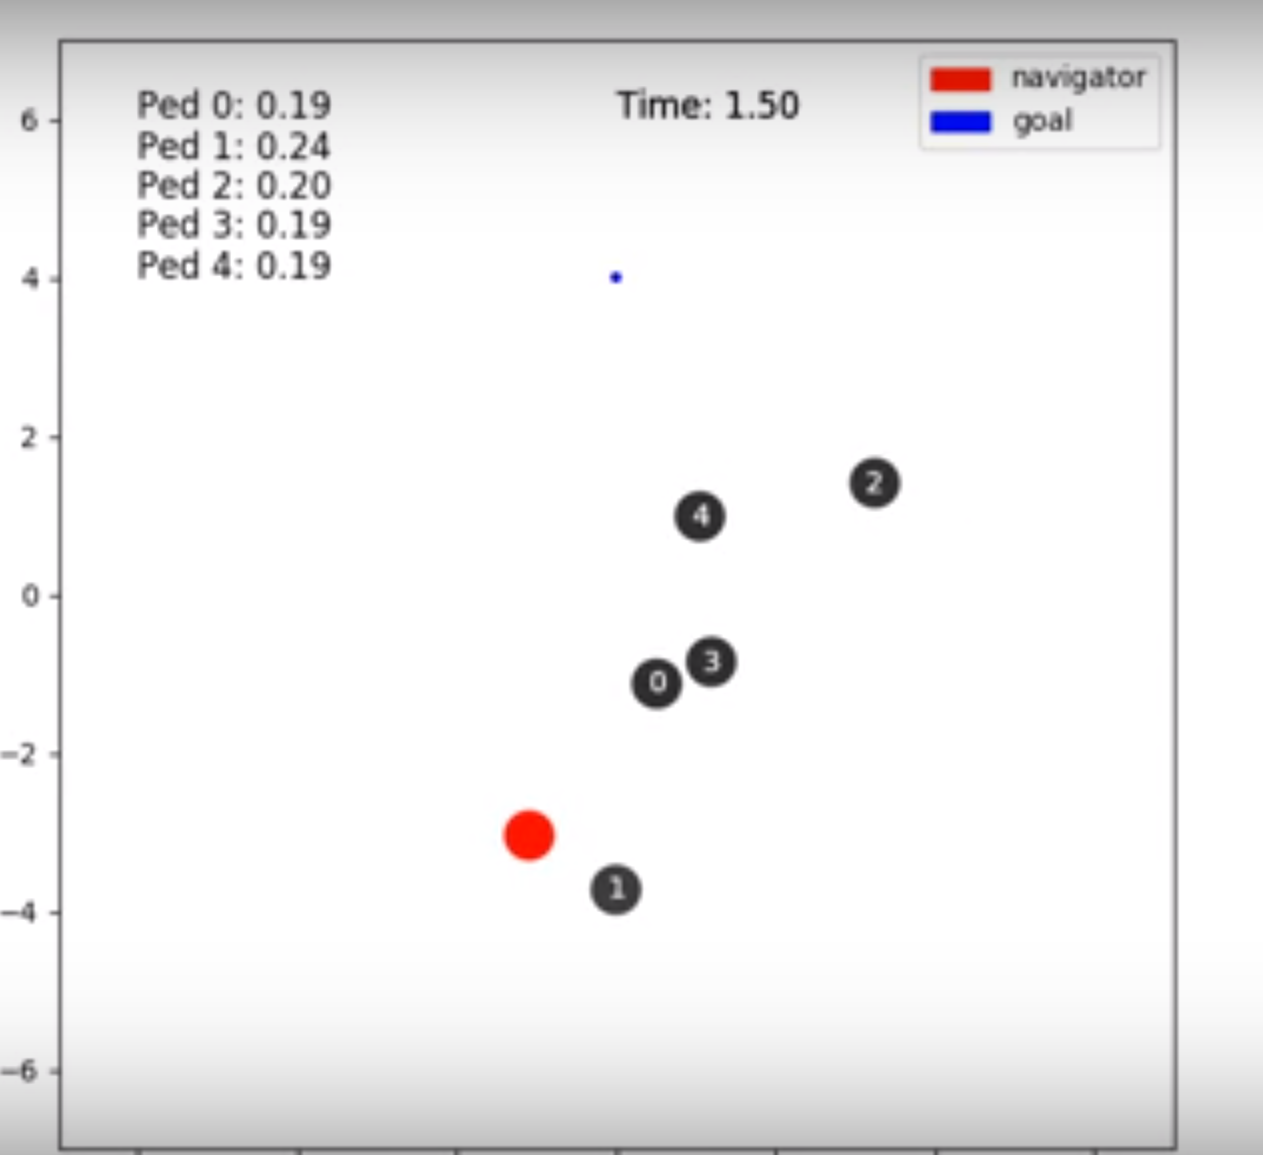
\includegraphics[width=0.2\textwidth]{figures/overview}
  \caption{Illustration of the socially compliant navigation in a crowded scene.}
  \label{fig:overview}
\end{figure}

Earlier works split the prediction and planning into two separate steps, attempting to identify a safe trajectory distant from the forecasted regions of the other agents for a few steps \cite{bennewitz_learning_2005,aoude_probabilistically_2013}. However, these untraversable regions can be very large in a crowded scene and cause the freezing robot problem \cite{trautman_unfreezing_2010}. To cope with it, jointly obstacle avoidance methods that plan the paths of all the interactive decision-makers simultaneously are proposed, in hope to make the navigation rooms cooperatively \cite{trautman_unfreezing_2010}. Though conceptually desirable, these methods suffer from the computational costs as well as the behavior stochasticity of the neighbors in practice. 

As an alternative, the reinforcement learning method has been used to train a policy that implicitly encodes the interactions and cooperations among agents. While great progress has been made in recent works \cite{chen_decentralized_2016,chen_socially_2017,long_towards_2017,everett_motion_2018}, existing models are limited in two aspects. i) The impact of a group of moving agents on the navigator is usually treated by a simplified model, such as, a maximum or LSTM operation, which discards some detailed information that might be important for modeling the crowd impact. ii) They are focused on the one-way interaction from the crowd to the navigator but omit the interactions within the crowd that can affect the state of each neighboring agent. These limitations may degrade the capacity of cooperative planning-based reasoning in complex and crowded scenes. 

In this work, we propose a novel pooling module for the reinforcement learning method, aiming to learn a socially compliant navigation policy in complex scenes. Inspired by \cite{alahi_social_2016,gupta_social_2018,vemula_social_2017}, we first extract the features of the pairwise social interaction between the navigator and each neighbor and subsequently use the soft attention to learn the importance of these interactions. In addition, we encode the impact of intra-interaction on each agent by a local occupancy map. Based on a social state concatenating these interactions, a navigator is trained to navigate through a crowd and learn a value network, which is used to evaluate the scenarios consisting of various group interactions and provide a cooperative navigation policy. An extensive set of experiments shows that our approach can effectively learn to soically compliant policy in crowded spaces, outperforming the state-of-the-art methods. 

\section{BACKGROUND} \label{sec:background} 

\subsection{Related Work}

RL, 
\vspace{2cm}

Social interaction, 
\vspace{2cm}

\subsection{Problem Formulation}

Consider a navigation task where the robot moves to an intended goal through a crowd of pedestrians $\{1,2,\dots,n\}$, which can be formulated as a decision making problem through a sequence of observations, action, and reward triplets\cite{chen_decentralized_2016,chen_socially_2017,everett_motion_2018}. Let $\bold{s}_t $ and $\tilde{\bold{s}}_t = [\tilde{\bold{s}}_t^1, \tilde{\bold{s}}_t^2, \dots, \tilde{\bold{s}}_t^n]$ denote the state of the robot and the pedestrians at time $t$ respectively. The full state of the robot is defined as $ \bold{s} = [\bold{p}, \bold{v}, r, \theta, \bold{p_g}, v_{pref}]$ and the observable state of a pedestrian is defined as $ \tilde{\bold{s}}_i = [\bold{p}, \bold{v}, r]$, where $\bold{p}=[p_x,p_y]$ and $\bold{v}=[v_x,v_y]$ are the vectors of location and velocity in the $2D$ plane, $r$ is the radius. We assume that the robot is aware of its heading angle $\theta$, goal position $\bold{p_g}$ and preferred speed $v_{pref}$ and the robot velocity can be achieved by the action command $\bold{u}_t$ immediately, $\bold{v}_t = \bold{u}_t$. 

The desired navigation policy, $\pi : (\bold{s}_t, \tilde{\bold{s}}_t) \mapsto \bold{u}_t$, is to maximize the objective function without violating the constraints:
\begin{subequations} \label{eq:optimization}
\begin{align}
& \underset{\pi(\bold{s}, \tilde{\bold{s}})}{\text{argmax}}
& & \mathbb{E}[\sum_{t=0}^T R_t | \bold{s}_0, \tilde{\bold{s}}_0, \bold{p}_g, \pi] \label{eq:obj} \\
& \text{subject to} 
& & \bold{p}_T = \bold{p}_g \label{eq:goal} \\
&&& \bold{p}_t = \bold{p}_{t-1} + \Delta t \pi(\bold{s}_{t-1}, \tilde{\bold{s}}_{t-1}) & t = 1, \dots, T \label{eq:kinematics} \\
&&& \left\Vert \bold{p}_t - \tilde{\bold{p}}_t^i \right\Vert >= r + \tilde{r}^i & i = 1, \dots, n \label{eq:safety}
\end{align}
\end{subequations}
where (\ref{eq:obj}) is the expected total reward that the robot can obtain in the navigation task, (\ref{eq:goal}) is the goal constraint, (\ref{eq:kinematics}) is the kinematics of the robot, (\ref{eq:safety}) is the safety constraint, $T$ is the time to reach the goal, and $\Delta t$ is the time step interval. 

The reward function is designed to penalize the collision and uncomfortable distance and award the accomplishment of the navigation task, 
\begin{equation}
    R(\bold{s},\tilde{\bold{s}},\bold{u})= 
\begin{dcases}
    -??? & \text{if} ~~ d < 0 \\
    -0.? + d? & \text{else if} ~~ d < 0.2 \\
    1 & \text{else if} ~~ \bold{p}=\bold{p}_g \\
    0 & \text{otherwise} 
\end{dcases}
\end{equation}
where $d$ is the seperation distance between the robot and the pedestrian within the time interval $\Delta t$. 

The problem (\ref{eq:optimization}) can be tackled by a reinforcement learning method, which seeks the optimal policy 
\begin{equation}
\pi^{*} = argmax [TODO]
\end{equation}
where $V^{*}$ is the optimal value function: 
\begin{equation}
V^{*} = 
\end{equation}
and $P $ is the transition dynamics. 

\section{APPROACH} \label{sec:approach} 

Formulation, 

\section{RESULTS} \label{sec:results} 

Simulation experiments, 

Real-world experiments, and video. 

\section{CONCLUSION} \label{sec:conclusion} 

In this paper, 

% \subsection{System Structure}

\addtolength{\textheight}{-10cm}   % This command serves to balance the column lengths
                                  % on the last page of the document manually. It shortens
                                  % the textheight of the last page by a suitable amount.
                                  % This command does not take effect until the next page
                                  % so it should come on the page before the last. Make
                                  % sure that you do not shorten the textheight too much.

\section*{ACKNOWLEDGMENT}

We would like to thank ... 

\bibliographystyle{IEEEtran}
\bibliography{vita-social-nav}

% \begin{thebibliography}{99}

% \end{thebibliography}

\end{document}


% @IEEEtranBSTCTL{IEEEexample:BSTcontrol,
%   CTLuse_url = "no",
%   CTLuse_article_number = "yes",
%   CTLuse_paper = "yes",
%   CTLuse_forced_etal = "yes",
%   CTLmax_names_forced_etal = "4",
%   CTLnames_show_etal = "1",
%   CTLuse_alt_spacing = "yes",
%   CTLalt_stretch_factor = "4",
%   CTLdash_repeated_names = "yes",
%   CTLname_latex_cmd = ""
% }